\documentclass[french]{article}
\usepackage[T1]{fontenc}
\usepackage[utf8]{inputenc}
\usepackage[a4paper,top=3cm,bottom=2cm,left=1.5cm,right=1.5cm,headheight=60pt]{geometry}
\usepackage{babel} % gestion de la langue
\usepackage{float} % gestion des images
\usepackage{graphicx} % gestion des images
\usepackage{lipsum} % remplissage de texte
%\usepackage[parfill]{parskip} % pas d'indentation en début de paragraphe
\usepackage{libertine} % police d'écriture
\usepackage{multicol} % double colonne
\usepackage{fancyhdr} % gestion des en-têtes / pieds de page
\usepackage{fourier-orns}
\usepackage{pgfornament}
\usepackage{url}
% ============ HEADER / FOOTER =======================
\fancypagestyle{hdr-normal}{
  \renewcommand{\headrulewidth}{0pt}
  \renewcommand{\footrulewidth}{0pt}
    \fancyhead[L]{\bsc{Machine Learning} \\[-5pt] \vhrulefill{1pt} \hspace{70pt} \ \\ 2019}%
    \fancyhead[C]{\bsc{Université de Rennes 1} \\[-5pt] \ \\ \bsc{UFR Sciences Économiques}}%
    \fancyhead[R]{\raisebox{-0.15\height}{
\includegraphics[scale=0.1]{img/logo_r1n.png}}}
    \fancyfoot[L]{}
    \fancyfoot[C]{}
    \fancyfoot[R]{\bf\thepage}
}
\pagestyle{hdr-normal} % application en-têtes/pieds de page à l'ensemble du document

% ============ DEFINITIONS ===========================
\renewcommand{\thempfootnote}{\arabic{mpfootnote}} % numérotation numérique des notes dans minipage
\makeatletter % épaisseur du vhrulefill
   \def\vhrulefill#1{\leavevmode\leaders\hrule\@height#1\hfill \kern\z@}
\makeatother
\renewenvironment{abstract} % édit du abstract/résumé
 {\par\noindent\textbf{\abstractname}\ \ignorespaces\\}
 {\par\medskip}
\renewcommand{\footnoterule}{\kern -3pt \hrule height 0pt \kern 2pt} % suppression ligne notes


\begin{document}

\noindent\begin{minipage}{\textwidth}

\ \\[20pt]

{\LARGE \bf Projet Machine Learning - Groupe 2} \\

{\large \bf Léo Dutertre\footnote{Master 2 PPE, Alternant Banque de France - Université de Rennes 1}, 
            Axel Gardahaut\footnote{Master 2 PPE - Université de Rennes 1}, 
            Guy Tsang\footnote{Master 2 PPE - Université de Rennes 1}}



\end{minipage}

\

\noindent E-mail: 

\null

\begin{abstract}
\lipsum[14]
\end{abstract}

\noindent Mots-clés : mot, mot, mot

\

\noindent \vhrulefill{1.5pt} ~\pgfornament[height = 0.6cm,symmetry=h]{84} ~ \vhrulefill{1.5pt}


\begin{multicols}{2}
\section{Introduction}

Une société d'assurance souhaite affiner sa capacité à tarifer ses contrats automobiles avec ses clients. L'objectif est de faire payer à chaque assuré son \og juste prix \fg{} (directement en lien avec le risque encouru par la société en assurant son client). Ainsi, à partir d'un jeu de données sur ses clients, le but sera de construire un modèle qui prédit, pour chaque assuré, sa probabilité de déposer une réclamation au cours de la prochaine année. Plus cette probabilité est élevée, plus la tarification sera élevée pour l'assuré.

Ceci constitue un problème classique de modélisation aboutissant à un score. La métrique d'évaluation des prédictions devra être pertinente à cette problématique, sachant que la base de données fournie présente un déséquilibre de la cible.

Le but de cet article scientifique est de présenter les données, la démarche du projet, les modèles de prédiction utilisés et enfin, les résultats obtenus.

\section{Données}

Les données sont fournies par la société d'assurance en question et fournissent des informations dans plusieurs domaines :

\begin{itemize}
    \item des variables concernent l'assuré en personne et sont repérées par le suffixe "ind" dans le nom,
    \item des variables concernent la région de l'assuré et sont repérées par le suffixe "reg" dans le nom,
    \item des variables concernent la voiture de l'assuré et sont repérées par le suffixe "car" dans le nom,
    \item des variables calculées, sans davantage de détails et sont repérées par le suffixe "calc" dans le nom.
\end{itemize}

La variable cible ("target" dans la base) est binaire et indique si une réclamation a été déposée ("1") par l'assuré ou non ("0"). Chaque ligne de la base de données correspond à un assuré automobile.

Une base d'apprentissage et une base de test sont directement fournies. L'apprentissage et la validation des modèles doit se faire sur la première base tandis que la seconde base ne doit intervenir à aucune phase de l'apprentissage. Celle-ci ne doit servir qu'à tester la performance du modèle retenu sur des nouvelles données. Des valeurs manquantes sont présentes dans les deux échantillons.

\section{Démarche du projet}

\subsection{Définition du cadre d'analyse}

Le projet débute par une mise au point sur les objectifs de la problématique. Il s'agit d'un problème de classification mais l'objectif s'arrête au scoring des clients. Le score correspond à la probabilité pour chaque client de déposer une réclamation dans l'année à venir. La métrique retenue pour évaluer la performance prédictive des modèles est celle du Coefficient Normalisé de Gini. Le coefficient de Gini permet de comparer la proportion cumulée des labels positifs prédits avec la proportion théorique. De plus, ce coefficient est directement lié à la courbe de Lorentz, souvent utilisée en Économie pour évaluer les inégalités salariales. Si on transpose ce concept à une société d'assurance (figure 1), on identifie l'intérêt principal de coefficient dans notre contexte.

Une lecture de la courbe de Lorentz (figure 1) serait \og les 15\% des assurés les plus risqués paient 90\% de l'ensemble des factures d'assurance \fg{}. Ceci correspond bien au principe de mutualisation des risques qui correspond à la base des systèmes d'assurance. Ainsi, plus le coefficient de Gini est élevé, plus la capacité à individualiser les tarifs sera bonne.

\begin{figure}[H] \centering
  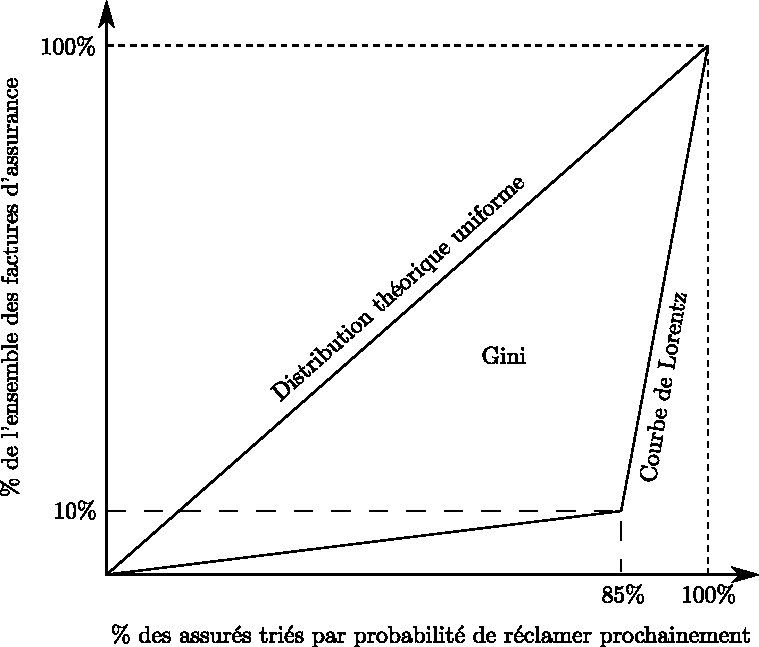
\includegraphics[width = \columnwidth]{img/gini}
  \caption{Coefficient de Gini et Courbe de Lorentz}
\end{figure}


La normalisation de ce coefficient permet de s'assurer que la valeur prise par la métrique va de 0 (aucune capacité prédictive) à 1 (capacité prédictive parfaite). Cette normalisation est fonction du taux de labels positifs dans l'échantillon.

\subsection{Statistiques Descriptives}

Les statistiques descriptives sont faites pour vérifier le type de données traitées, la présence de valeurs manquantes, la présence de valeurs aberrantes et les distributions. On discerne alors les variables qui présentent des valeurs manquantes et à quelle mesure. De plus, on repère les types de variables (continues, catégorielles, ordinales, etc.) pour spécifier le traitement au cas par cas.

L'inférence faite à partir de modalités rares (moins de 5\% en général) n'est pas robuste et peut conduire à du sur-apprentissage. Les statistiques descriptives sur les variables catégorielles permet de détecter ces modalités pour les traiter ensuite.

Enfin, l'étude des variables continues permet de prévoir l'utilité de transformations telles qu'une normalisation ou une standardisation afin de rapporter les valeurs à une même échelle.

\subsection{Benchmark d'ouverture}

Il est intéressant de placer un benchmark afin d'avoir une valeur de la métrique objectif (Coefficient Normalisé de Gini) à dépasser. Ce benchmark étant fait dès le départ du projet, sans traitement préalable sur les données, permet d'avoir un seuil à dépasser grâce aux traitements et à l'enrichissement de l'information faits sur les données.

Le score obtenu par un Light GBM\footnote{Gradient Boosting Machine} est généralement élevé et rapidement obtenu. Celui-ci est de : 0.2719186 par validation croisée sur 5 folds.

Bien que le score obtenu est sujet à fluctuer, il est intéressant de refaire un Light GBM après chaque étape de traitement pour voir si les modifications apportées augmente ou diminue le score. Il s'agit uniquement d'une valeur de référence, elle ne permet pas de valider l'intérêt ou non d'un traitement à l'exception si elle diffère de façon significative de la précédente valeur.


\subsection{Pré-traitement des données}

Le pré-traitement des données consiste essentiellement à la gestion des valeurs manquantes. Plusieurs variables ont été identifiées dans les statistiques descriptives (figure 2). Selon le taux de valeurs absentes, la manipulation appliquée sera différente. 

\begin{figure}[H] \centering
  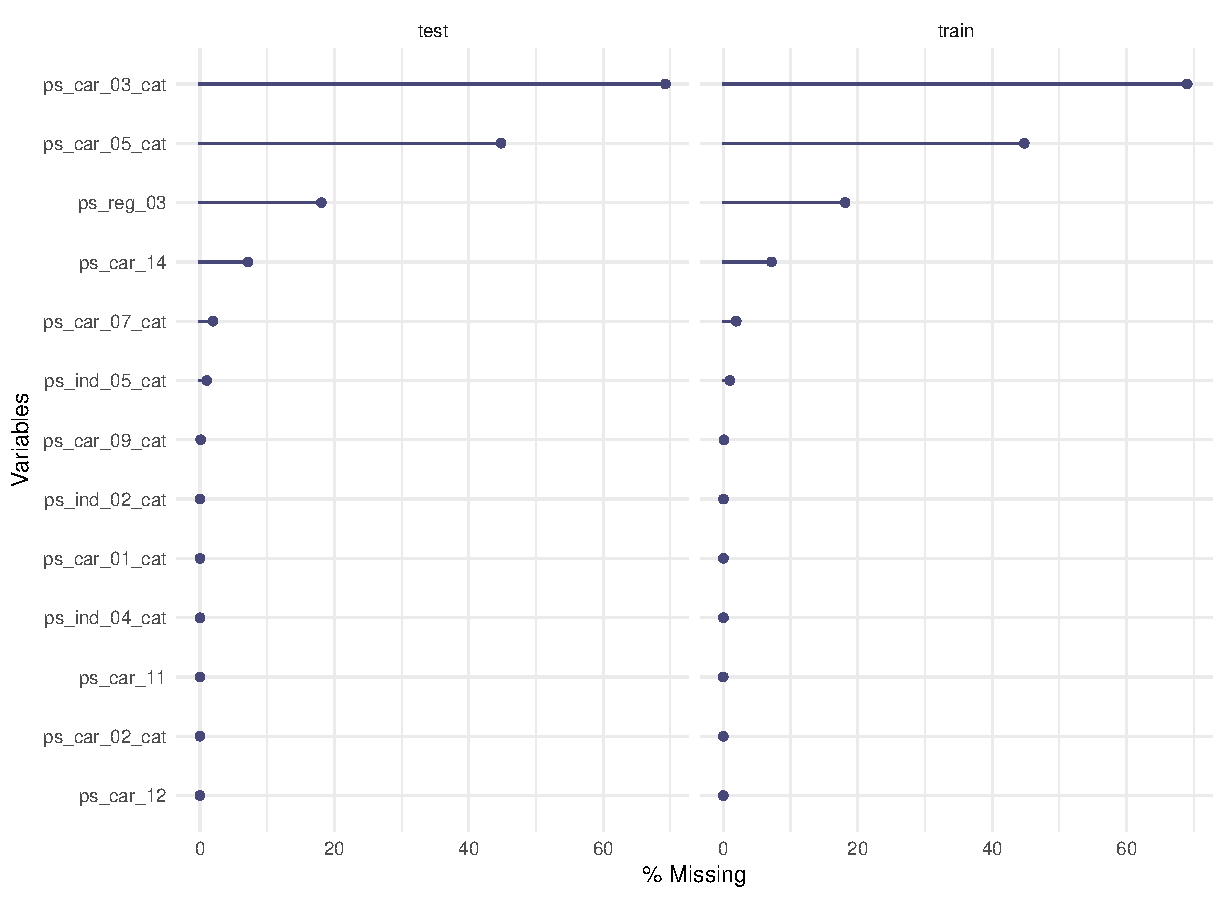
\includegraphics[width = \columnwidth]{img/missing_values}
  \caption{Valeurs manquantes}
\end{figure}


Deux colonnes présentent trop de valeurs manquantes (plus de 40\%) pour une imputation sophistiquée, ainsi, elles sont remplacées par une valeur spéciale (-999 par exemple) pour conserver l'information issue de l'absence de valeur. En effet, en croisant ces variables avec la cible, il est noté que le taux croisé d'effectif est significativement différent à ceux des valeurs normales.

Pour le reste des variables, une imputation par forêt aléatoire est faite. Le procédé d'imputation est le suivant :
\begin{itemize}
    \item Utiliser uniquement l'échantillon d'apprentissage pour construire la forêt aléatoire.
    \item Modéliser la variable étudiée en s'assurant qu'il s'agisse du bon type d'arbres (classification ou régression) en utilisant les autres variables comme régresseurs.
    \item Prédire les valeurs de la variable étudiée pour l'ensemble des observations manquantes des deux échantillons (apprentissage et test).
    \item Remplacer les valeurs manquantes et s'assurer qu'il n'y a plus de valeurs manquantes pour la colonne traitée.
\end{itemize}

Suite aux imputations faites, le Light GBM de référence renvoie un Gini de 0.2721429, toujours par validation croisée sur 5 folds. On note une augmentation par rapport au benchmark bien que la différence est trop faible pour en tirer des conclusions.

\subsection{Sélection des variables}

Le Light GBM effectué après les imputations permet également d'identifier l'importance des variables dans le pouvoir prédictif du modèle. L'importance d'une variable peut être mesurée de différentes manières. Celle adoptée ici est le \og Gain \fg{}. Il s'agit de la contribution de la variable au modèle, calculé en sommant la contribution associée à chaque arbre du modèle. Ainsi, plus une variable contribue au pouvoir prédictif d'un modèle, plus son \og Gain \fg{} associé sera élevé. On récupère la première moitié des variables les plus importantes au modèle.

\begin{figure}[H] \centering
  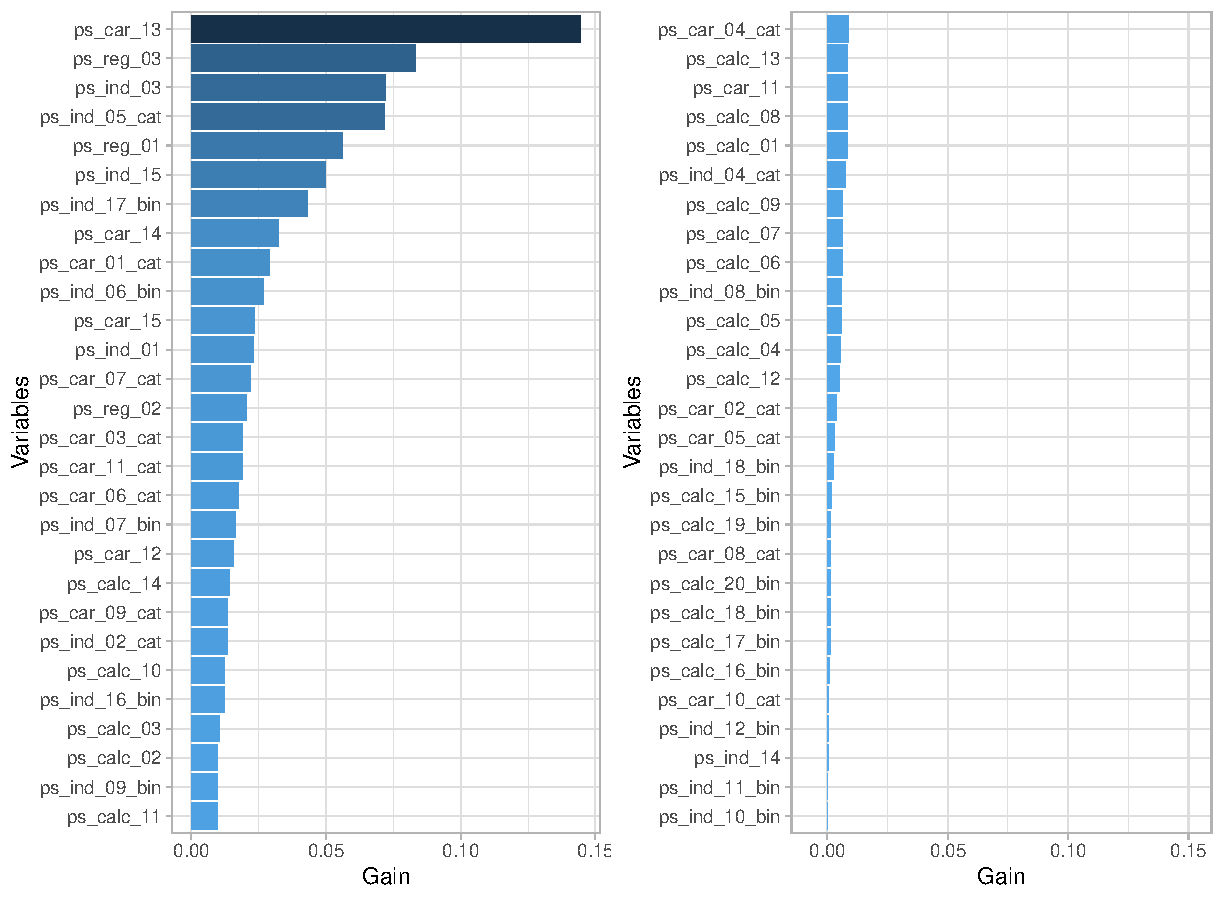
\includegraphics[width = \columnwidth]{img/var_imp_lgb}
  \caption{Importance des variables}
\end{figure}


En plus des importances issues du Light GBM, une forêt aléatoire (non paramétrée de façon optimale) est construite pour y sortir une autre liste d'importance ("\og permutation \fg{} qui est équivalente au \og Gain \fg{}). De même, cette seconde liste est issue de la première moitié des variables les plus importantes au modèle.

De façon globale, les deux listes coïncident, avec quelques exceptions et l'union de ces deux listes constitue la liste finale des variables retenues pour la suite. Au total, ce sont 33 régresseurs qui sont retenus. On passe alors de 57 prédicteurs à 33.

\subsection{Traitement des données}

Lors de la phase des statistiques descriptives, plusieurs variables présentaient des modalités rares (effectif inférieur à 5\%). Celles-ci doivent être fusionnées pour pouvoir inférer des résultats robustes.

La stratégie de fusion peut passer par une projection des modalités d'une variable sur le premier plan factoriel d'une AFDM. Chaque modalité rare sera alors associée à la modalité fréquente la plus proche d'elle (et si possible projetée dans la même direction), ou un ensemble de modalités rares peuvent se regrouper pour former un groupe supplémentaire (clusters).

Autrement, la stratégie peut passer par des tableaux de contingence qui croisent les variables problématiques avec la cible. Les modalités rares sont fusionnées soit entre elles si elles se comportent de façon similaire, soit avec une modalité fréquente si le comportement s'y rapproche.

\subsubsection{Fusion des modalités rares par AFDM}

La fusion de modalités est laissée à l'appréciation du statisticien.

\begin{figure}[H] \centering
  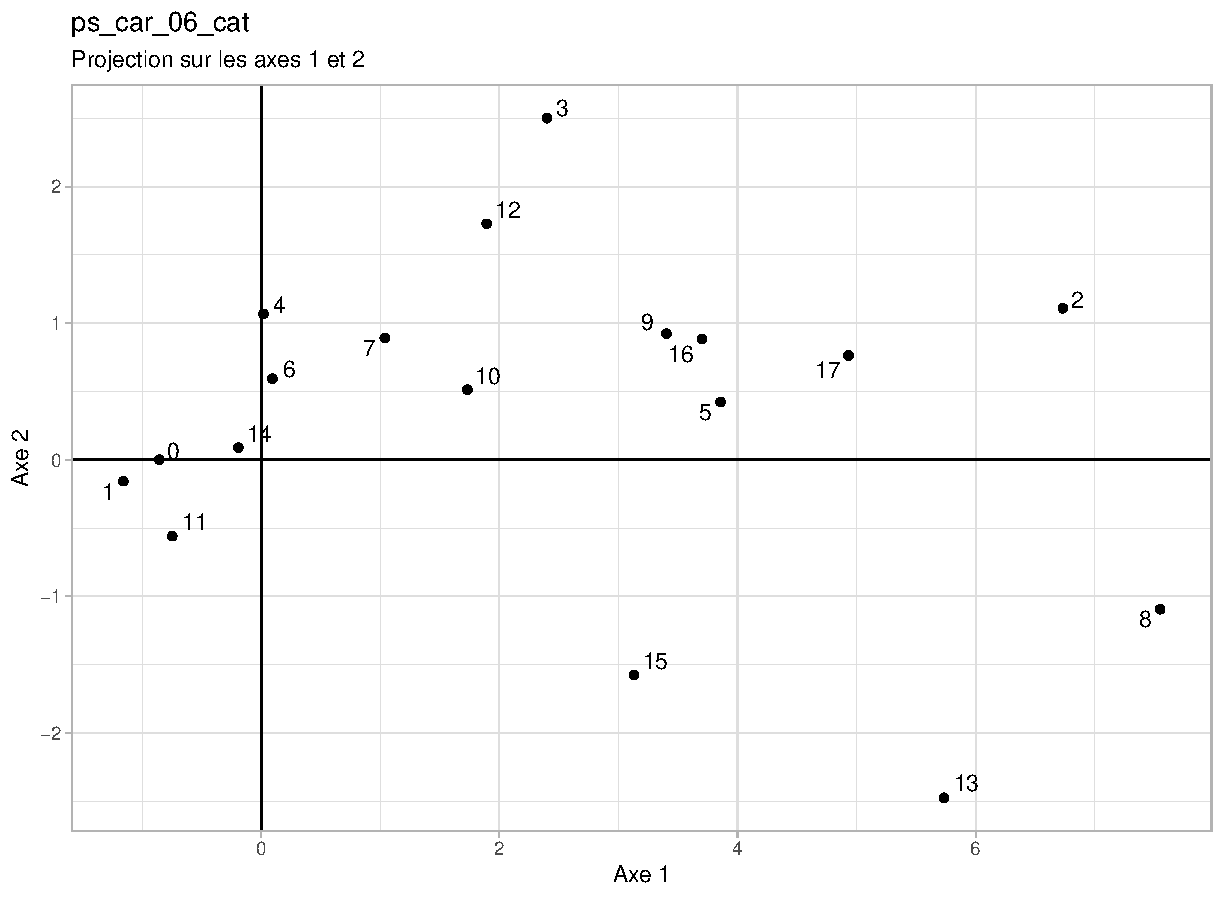
\includegraphics[width = \columnwidth]{img/ex_afdm}
  \caption{Exemple de projection de modalités par AFDM}
\end{figure}

\subsubsection{Fusion des modalités rares par tableaux croisés}

La fusion de modalités est laissée à l'appréciation du statisticien.

\begin{figure}[H] \centering
  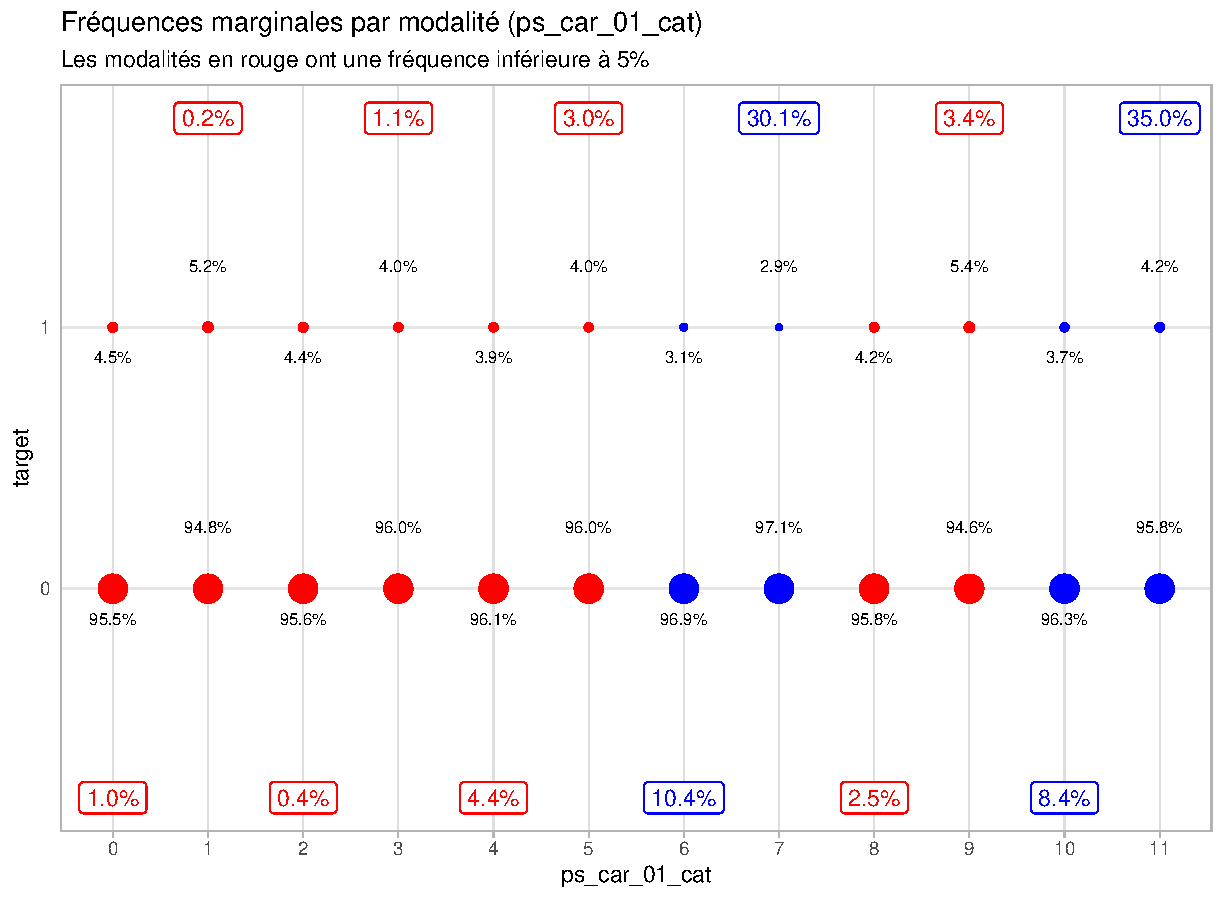
\includegraphics[width = \columnwidth]{img/ex_tabc}
  \caption{Exemple de projection de modalités par croisement}
\end{figure}

\[ * \ * \ * \]

Une variable présente un grand nombre de modalités (104). Plutôt que de fusionner ces modalités, on peut s'en servir comme régresseur unique d'une régression logistique avec la variable cible comme variable à expliquer. Les modalités seront alors remplacées par les coefficients estimés et la variable deviendra alors numérique et continue.

Le Light GBM fournit un score de 0.2728841 (5fCV) pour la stratégie par AFDM et de 0.2756634 (5fCV) pour la stratégie par tableaux croisés. Le score ayant fortement augmenté pour la seconde stratégie, elle sera retenue pour la suite.

\subsubsection{Normalisation des données}

Certaines variables continues ont une distribution qui se rapprochent d'une distribution normale. Il serait intéressant de tenter de les normaliser à travers différentes méthodes (box-cox, logarithme, racine carré). Dans la figure suivante (figure 6), la distribution initiale n'est pas représentée car elle est trop éloignée de celle d'une loi normale.

\begin{figure}[H] \centering
  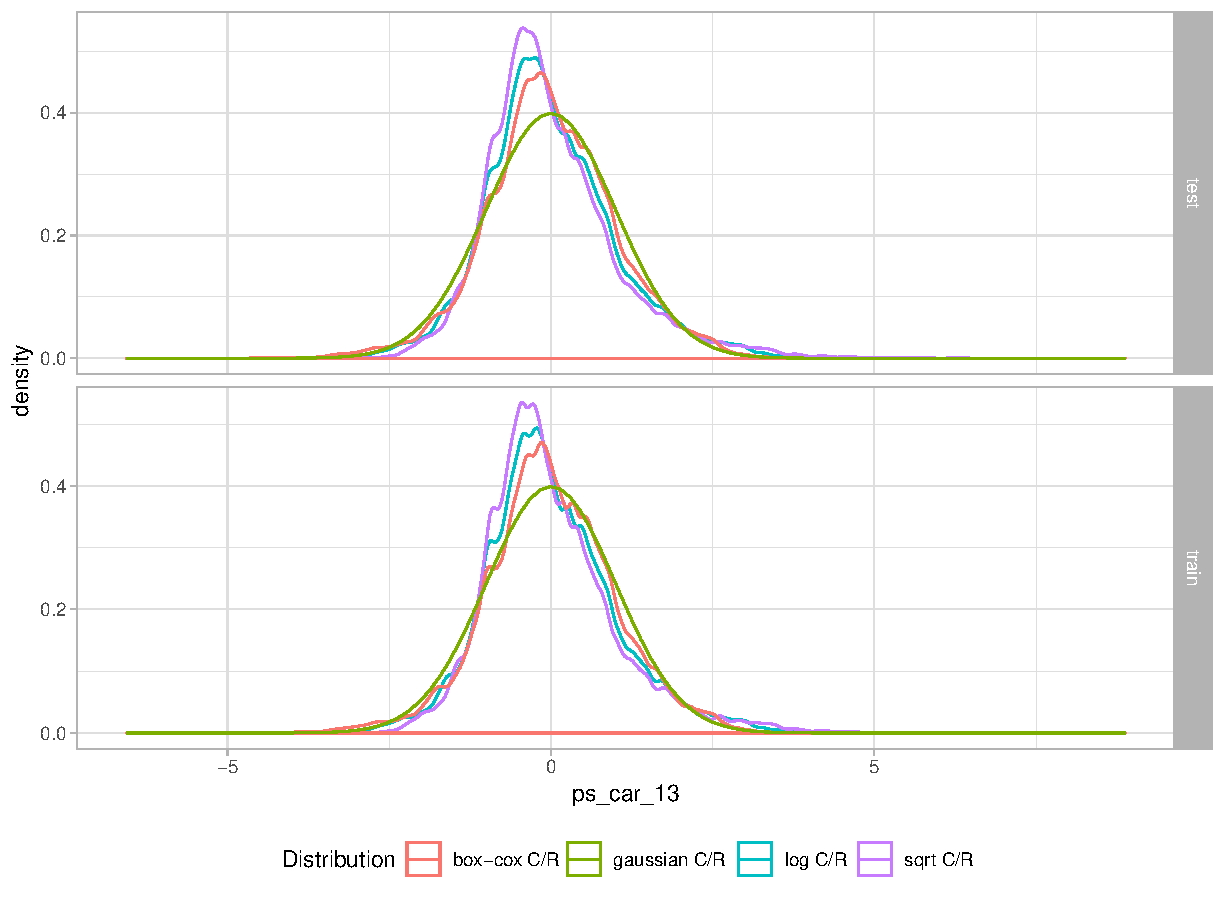
\includegraphics[width = \columnwidth]{img/ex_normalisation}
  \caption{Exemple de normalisation}
\end{figure}

Il est notable que la transformation de box-cox est la meilleure pour normaliser cette distribution. Cette étude est menée pour les variables continues.

En réutilisant un Light GBM pour mesurer les conséquences des normalisations faites, il est noté que la métrique diminue, suite à chacune des deux stratégies de fusion de modalités. On passe respectivement à un Gini de 0.2728511 (AFDM) et 0.2751949 (tableaux croisés). Ces diminutions sont minimes mais la normalisation des variables n'est pas obligatoire. Par conséquent, cette étape est laissée de côté pour la suite. 

À la fin de cette étape, le traitement se résume à la fusion de modalités en utilisant des tableaux de contingence.

\subsection{Étude des corrélations et dépendances}

L'objectif de cette étape est de diminuer à nouveau de nombre de variables explicatives. La stratégie est différente : il s'agit d'étudier les corrélations et les dépendances entre variables puis contre la cible. Ceci permet de détecter des problèmes de colinéarité et ou dépendance entre prédicteurs :

\begin{itemize}
    \item les liens entre variables continues se font grâce aux corrélations,
    \item les liens entre les variables continues et la cible se font grâce à un test d'ANOVA,
    \item les liens entre variables catégorielles (et la cible) se font grâce aux V de Cramer\footnote{Le V de Cramer est la statistique du $\chi^2$ standardisée de façon à ce qu'elle varie entre 0 et 1}.
\end{itemize}

Les variables qui dépassent les seuils arbitrairement fixés ou qui ne passent pas le test d'ANOVA sont laissées de côté. Le nombre de prédicteurs chute alors à 29.

\subsection{Paramétrisation des modèles}

Une dizaine d'algorithmes sont testés pour tenter d'avoir le meilleur pouvoir prédictif. On y trouve des modèles de base (LDA, KNN, régression logistique (pénalisée), SVM), puis des modèles de bagging (RF) et de boosting (ADABoost, GBM, XGBM, LGBM).

L'ensemble des modèles ensemblistes et la régression logistique pénalisée sont optimisés selon leurs paramètres de pré-apprentissage\footnote{Les algorithmes KNN et SVM ne sont pas optimisés faute du temps d'exécution nécessaire au calcul de matrices immenses de distance}.

Pour chaque modèle, la question du ré-échantillonnage est traitée. Pour l'ensemble des modèles, les stratégies de down-sampling, up-sampling et SMOTE sont testées en plus du cas sans sampling.

\section{Résultats}

\begin{figure}[H] \centering
  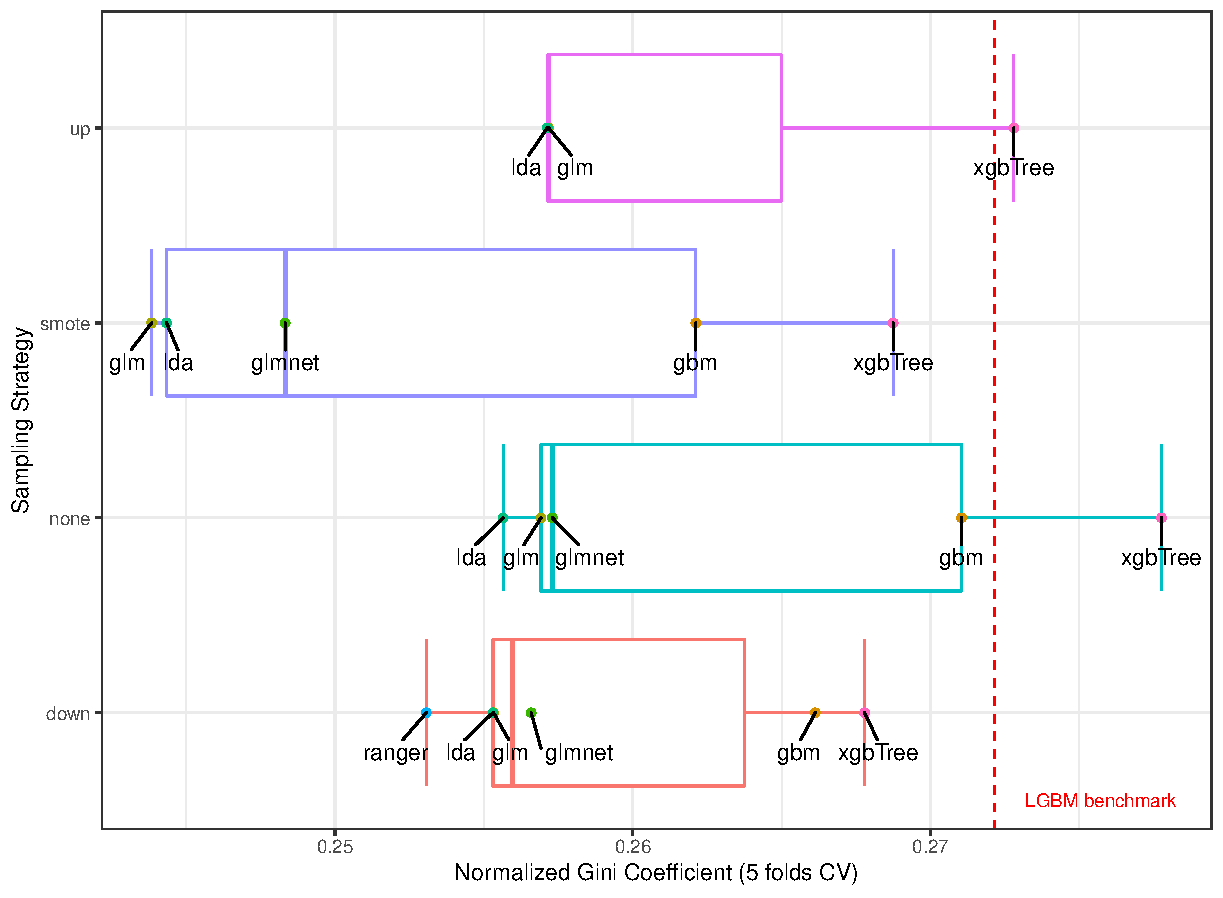
\includegraphics[width = \columnwidth]{img/results}
  \caption{Résultats}
\end{figure}

% références
\nocite{*}
\bibliographystyle{acm}
\bibliography{biblio}

\end{multicols}

\end{document}

